\documentclass[%
  crop,%
  tikz,%
  multi=false%
]{standalone}%
\usepackage[utf8]{luainputenc}%
\usepackage[no-math]{fontspec}%
\defaultfontfeatures{%
  Numbers={OldStyle,Proportional},%
  Ligatures=TeX,%
  Extension=.ttf,%
}%
\setmainfont[%
  UprightFont=*-Regular,%
  ItalicFont=*-Italic,%
  BoldFont=*-Bold,%
  BoldItalicFont=*-BoldItalic,%
]{Raleway}%
\setsansfont[%
  UprightFont=*-Regular,%
  ItalicFont=*-Italic,%
  BoldFont=*-Bold,%
  BoldItalicFont=*-BoldItalic,%
]{Raleway}%
\usepackage[frenchmath]{mathastext}%
\usepackage{amsmath}%
\usepackage{amssymb}%
\usepackage{mathrsfs}%
\usepackage{mathtools}%
\usepackage{siunitx}%
\usepackage[siunitx]{circuitikz}%
\usetikzlibrary{calc,backgrounds,arrows.meta,patterns,positioning}%
\ctikzset{bipoles/length=1.2cm}%

% Colors
\usepackage{xcolor}%
\definecolor{RoseauGreen}{HTML}{cad40e}%
\definecolor{RoseauGrey}{HTML}{adb9cb}%
\definecolor{RoseauBlue}{HTML}{234e83}%

\DeclareMathOperator{\sign}{sign}%

% Sets
\let\C\relax
\newcommand{\R}{\ensuremath{\mathbb{R}}} % Real
\newcommand{\N}{\ensuremath{\mathbb{N}}} % Natural
% \newcommand{\C}{\ensuremath{\mathbb{C}}} % Complexes
\newcommand{\B}{\ensuremath{\mathscr{B}}} % Electrical buses
\newcommand{\Ch}{\ensuremath{\mathscr{C}}} % Loads
\renewcommand{\L}{\ensuremath{\mathscr{L}}} % Lines
\renewcommand{\P}{\ensuremath{\mathscr{P}}} % Phases

% Phases
\newcommand{\arm}{\ensuremath{\mathrm{a}}}%
\newcommand{\brm}{\ensuremath{\mathrm{b}}}%
\newcommand{\crm}{\ensuremath{\mathrm{c}}}%
\newcommand{\nrm}{\ensuremath{\mathrm{n}}}%
\newcommand{\grm}{\ensuremath{\mathrm{g}}}%
\newcommand{\abrm}{\ensuremath{\mathrm{ab}}}%
\newcommand{\bcrm}{\ensuremath{\mathrm{bc}}}%
\newcommand{\carm}{\ensuremath{\mathrm{ca}}}%
\newcommand{\anrm}{\ensuremath{\mathrm{an}}}%
\newcommand{\bnrm}{\ensuremath{\mathrm{bn}}}%
\newcommand{\cnrm}{\ensuremath{\mathrm{cn}}}%
\newcommand{\agrm}{\ensuremath{\mathrm{ag}}}%
\newcommand{\bgrm}{\ensuremath{\mathrm{bg}}}%
\newcommand{\cgrm}{\ensuremath{\mathrm{cg}}}%
\newcommand{\ngrm}{\ensuremath{\mathrm{ng}}}%
\newcommand{\abcrm}{\ensuremath{\mathrm{abc}}}%
\newcommand{\abcnrm}{\ensuremath{\mathrm{abcn}}}%

% Transformer
\newcommand{\Xrm}{\ensuremath{\mathrm{X}}}%
\newcommand{\Yrm}{\ensuremath{\mathrm{Y}}}%
\newcommand{\Zrm}{\ensuremath{\mathrm{Z}}}%
\newcommand{\xrm}{\ensuremath{\mathrm{x}}}%
\newcommand{\yrm}{\ensuremath{\mathrm{y}}}%
\newcommand{\zrm}{\ensuremath{\mathrm{z}}}%
\newcommand{\Arm}{\ensuremath{\mathrm{A}}}%
\newcommand{\Brm}{\ensuremath{\mathrm{B}}}%
\newcommand{\Crm}{\ensuremath{\mathrm{C}}}%
\newcommand{\Nrm}{\ensuremath{\mathrm{N}}}%

% Indices or exponents
\newcommand{\cons}{\ensuremath{\mathrm{cons.}}}%
\renewcommand{\prod}{\ensuremath{\mathrm{prod.}}}%
\newcommand{\theo}{\ensuremath{\mathrm{th.}}}%
\newcommand{\const}{\ensuremath{\mathrm{const.}}}%

% Variables
\newcommand{\umax}{\ensuremath{U^{\max}}}%
\newcommand{\umaxnorm}{\ensuremath{U^{\max\,\text{norm.}}}}%
\newcommand{\umin}{\ensuremath{U^{\min}}}%
\newcommand{\uminnorm}{\ensuremath{U^{\min\,\text{norm.}}}}%
\newcommand{\unom}{\ensuremath{U^{\text{nom.}}}}%
\newcommand{\unomnorm}{\ensuremath{U^{\text{nom.}\,\text{norm.}}}}%
\newcommand{\uup}{\ensuremath{U^{\text{up}}}}%
\newcommand{\uupnorm}{\ensuremath{U^{\text{up}\,\text{norm.}}}}%
\newcommand{\uupprime}{\ensuremath{U^{\text{up}\,\prime}}}%
\newcommand{\udown}{\ensuremath{U^{\text{down}}}}%
\newcommand{\udownnorm}{\ensuremath{U^{\text{down}\,\text{norm.}}}}%
\newcommand{\udownprime}{\ensuremath{U^{\text{down}\,\prime}}}%
\newcommand{\smax}{\ensuremath{S^{\max}}}%
\newcommand{\pmax}{\ensuremath{P^{\max}}}%
\newcommand{\sproj}{\ensuremath{\underline{S^{\text{proj.}}}}}%
%

\begin{document}
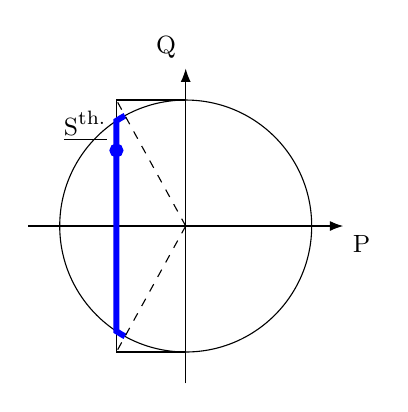
\begin{tikzpicture}[%
    show background rectangle,%
    tight background,%
    background rectangle/.style={fill=white}%
  ]
  %
% Styles
%
\tikzset{every node/.style={font=\small}};%
\tikzset{fleche/.style={->, -{Latex}}};%
\tikzset{point/.pic={\filldraw[#1] (0,0) circle[radius=0.05];}};%
\tikzset{domaine/.style={blue, line width=0.75mm}};%
\tikzset{domaine hache/.style={domaine, pattern=north east lines, pattern color=blue}};%

%
% Macros
%
\pgfmathsetmacro{\r}{1.6};%
\pgfmathsetmacro{\R}{2};%
\pgfmathsetmacro{\pthvaleur}{-0.55*\r};%
\pgfmathsetmacro{\qthvaleur}{0.6*\r};%
\pgfmathsetmacro{\angthvaleur}{acos(\pthvaleur/\r)}%
\pgfmathsetmacro{\angeuclthvaleur}{180+atan(\r/\pthvaleur)}%
\pgfmathsetmacro{\qthmaxvaleur}{\r*sin(\angthvaleur)}%

%
% Common part of the picture
%
\draw (0,0) circle[radius=\r];%
\draw[fleche] (-\R,0) -- (\R,0) node[below right] {$P$};%
\draw[fleche] (0,-\R) -- (0,\R) node[above left] {$Q$};%
\node[above left] at (\pthvaleur,\qthvaleur) {$\underline{S^{\theo}}$};%
\draw (0,-\r) -- (\pthvaleur,-\r) -- (\pthvaleur,\r) -- (0,\r);%
% Local Variables:
% mode: latex
% TeX-engine: luatex
% TeX-source-correlate-method-active: synctex
% ispell-local-dictionary: "british"
% coding: utf-8
% LaTeX-indent-level: 2
% fill-column: 120
% End:
%

  % The domain is a segment with two arc circle
  \draw[domaine] (-\angeuclthvaleur:\r) arc[start angle=-\angeuclthvaleur, end
      angle=-\angthvaleur, radius=\r] -- (\pthvaleur,\qthmaxvaleur) arc [start angle=\angthvaleur, end
      angle=\angeuclthvaleur, radius=\r];%

  \pic[domaine] at (\pthvaleur,\qthvaleur) {point};%

  \draw[dashed] (0,0) -- (\pthvaleur,\r);%
  \draw[dashed] (0,0) -- (\pthvaleur,-\r);%
\end{tikzpicture}
\end{document}
% Local Variables:
% mode: latex
% TeX-engine: luatex
% TeX-source-correlate-method-active: synctex
% ispell-local-dictionary: "british"
% coding: utf-8
% LaTeX-indent-level: 2
% fill-column: 120
% End:
